\section{Driving support systems}

In this document we are mainly concerned about driving assistance systems. Such system facilitates the task of driving. This support can appear in several forms: 

\begin{itemize}
\item visual alerts
\item auditory alerts
\item tactile alerts (also known as haptics\cite{riener2010sensor})
\end{itemize}

Driving support system may also provide support in a less passive manner as well:

\begin{itemize}
\item change how the car respond to the drivers commands for assisting a maneuver
\item change how the car behaves, with partial or fully automatic command
\end{itemize}

This field has gained several adepts. Automotive industry and researchers are studying it thoroughly these days.

Thus, driving support systems and its applications are becoming a popular tool. To exemplify such change, some countries changed their laws to make mandatory that all new cars manufactured have a given support system installed as a minimum equipment, ABS(Anti-lock break systems)  for instance \footnote{http://www.estadao.com.br/noticias/impresso,freio-abs-passa-a-ser-obrigatorio,351726,0.htm}.

One of the reasons for such change is the increasing number of incidents involving vehicles. \textbf{Risk of incidents} is growing as the population of cars grows, and there is no signal in changing those numbers in next years, so driving support systems is coping with task of making the car a safer transportation system, among others tasks (Figure~\ref{fig:sensor:target}).

Those incidents may be related with the cognitive capacity limitation of the human being. With the goal of quantify this capacity, a research conducted in 2008 studied the human cognitive limitation for visual sensing mechanism \cite{LautarutisV}. This report established the limit number of objects which the human is capable of track simultaneously. This study establishes the limit of the human vision by associating it with the information channel capacity theorem (Shannon's theorem). 

Although this seems to be distant from our goal (safety), this research underlies the limitation of human driving skills. With it we can conclude that above certain number of surrounding vehicles, we may start to ignore the risk of collision with some vehicles that still may represent a risk. Besides, several factors can affect its behavior like fatigue, cognitive capacity or simply bad decisions.

%Although, cognition is not an absolute number it varies according to several parameters, like mental health, type of sensing mechanism (visual, auditory, tactile), amount of information transmitted, etc. 

The action of driving did not change considerably since its creation but several mechanisms to support the driver have been included in the vehicle. All to provide a comfortable and safer experience for the driver\cite{riener2010sensor}.

A more modern approach of driving support system has appeared: Advanced Driver Assistance Systems (ADAS). 

ADAS relies in computerized systems to process informations provided by the car (through sensors) to improve the user experience. 

ADAS is split in different research branches, each of them with its own applications and goals. Among those different branches (Figure \ref{fig:sensor:target}), our work will concentrate in supporting applications situated in \textbf{safety} branch. 

The goal of this work is to tackle a very common issue in safety application (object classification) and \textbf{not} develop an application.

This will be done by providing a theoretical framework to classify the environment in a high level manner, separating static and dynamic parts with the information acquired from the sensors.

\begin{figure}[h]
\centering
	\begin{tabular}{lr}\\
		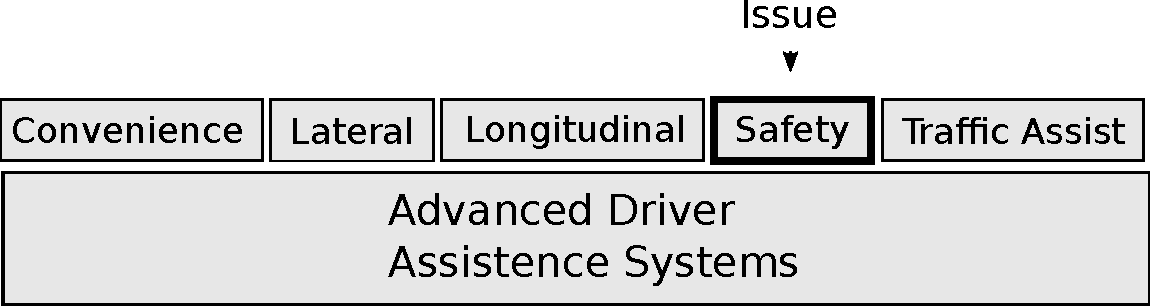
\includegraphics[scale=0.7]{img/fig:sensor:target} 
	\end{tabular}
	\caption{ADAS application stack and problem to be tacked (adapted from \cite{riener2010sensor})}
	\label{fig:sensor:target}
\end{figure}

Advanced Driver Assistance Systems rely on the perception. An ADAS works somehow similar to the human cognition, it requires a mean to perceive the environment before dispatch any action. 

There are different ways of perceiving the environment, usually we observe specific features, like: lighting, appearance, shapes, etc. Every feature requires a mechanism to process the information and convert the physical characteristics into electronic signal. The peripherals responsible for this process are called sensors, which will be discussed in more details in the Section \ref{sec:sensors}.

%% reviewed until here

\subsection{Sensors}
\label{sec:sensors}

%maybe replace the world system in the diagram and text by "control systems"

Sensing is the input for numerous biological systems (\textit{e.g.} nervous system, digestive system), enabling such systems to respond properly to the information provided by such sensors(eye, skin, etc.). 

This scheme is as important to robotics as they are for human being. In order to interact with the environment, a robot needs first to perceive it. This is done by capturing specific features, or at least some of them. The features observed depends on the application needs.

\begin{figure}[h]
   \centering
     \begin{tabular}{lr}
       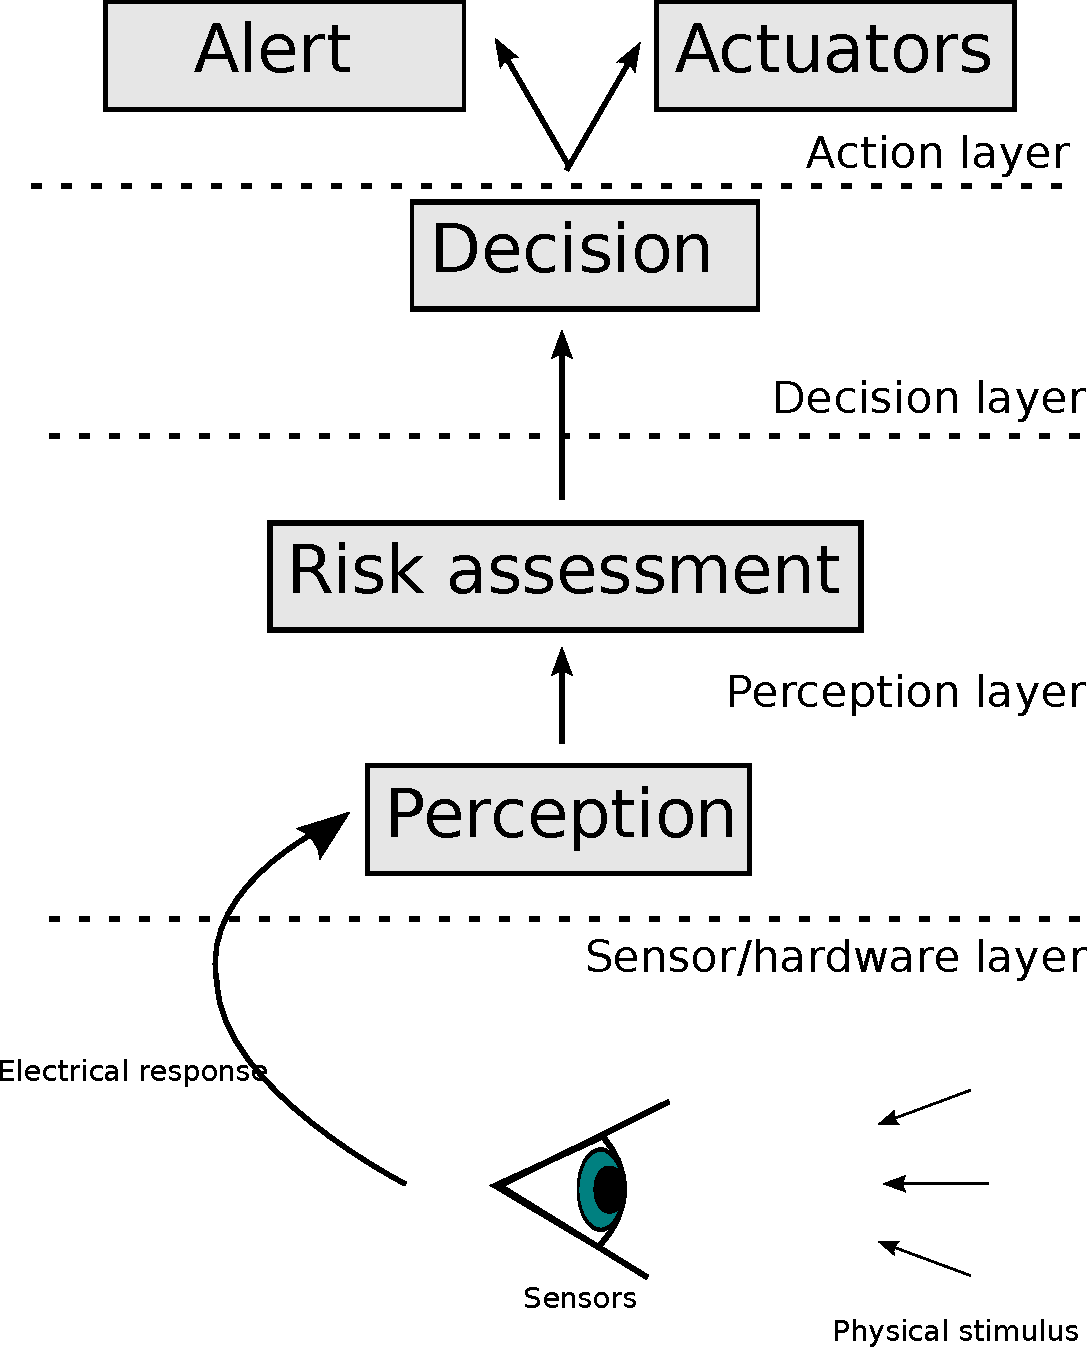
\includegraphics[scale=0.45]{img/fig:sensors:roles}
     \end{tabular}
   \caption{A general architecture of a system attached to sensors}
   \label{fig:sensors:role}
 \end{figure}

Sensors are the means in which complex systems acquire information about the environment. Although, the sensors play a key role in almost every systems. It is not their role to process information, only acquire them (Figure \ref{fig:sensors:role}). 

The sensors are normally incapable to respond to external stimulus without a system to process the data provided by it, and act. The system reacts to the sensor stimulus through other means.

Thus, a sensor is responsible for the data acquisition (electric interpretation of a physical stimulus). This data is directed to a perception layer which is allocated in an upper layer, which is responsible for the understanding of the environment and the objects located in it. 

In the \textit{risk assessment layer} is where the decisions are taken, this turns it into the main layer for the actual result of the safety application.

\subsubsection{Types}

There are virtually sensors for all kinds of properties (Figure~\ref{fig:sensors}) that we want to observe. In some literatures those properties can be called \textbf{measurands}\cite{riener2010sensor}. 

There exists two sets of classifications for sensors, they can be Proprioceptive/Exteroceptive with respect to the type of measurands \cite{iyengar1991autonomous} and they are classified in the manner how the measurands are obtained, which can be in a passive or active \cite{Hebert_2000_3595} manner. Active sensors emit energy to the environment so the measurand can be collected, a passive sensor is capable of observing the measurand without emit any type of energy in the environment.

Active and passive type refer to the electronic means in which the measurand is obtained. A second sensor typing is defined according to the target subject of the measurand, they can be proprioceptive and exteroceptive.

\textit{Proprioceptive} evaluate the ego-robot properties, giving informations about some \textbf{measurand} of the robot itself. Motor speed, payload, robot joint angles, battery voltage are some examples.  Inertial Measurement Unit (IMU) is a \textit{proprioceptive} sensor that observes the orientation, velocity and gravitational forces of the robot, it is a very common type of sensor and largely applied in robotics and in aviation.

\textit{Exteroceptive} gives information about the environment in which the robot is located. Thus, they extract useful environmental features. Light intensity and sound amplitude are some examples of \textit{exteroceptive} sensor.

\begin{figure}[h]
   \centering
     \begin{tabular}{lr}
       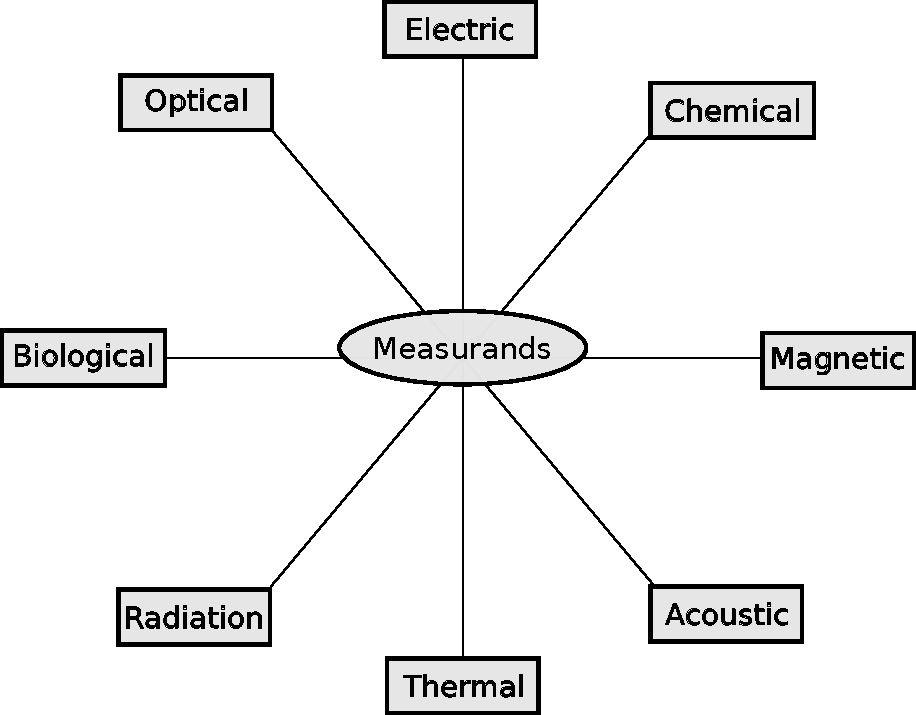
\includegraphics[scale=0.70]{img/fig:sensors}
     \end{tabular}
   \caption{Different types of measurands (adapted from \cite{WhiteRichard})}
   \label{fig:sensors}
 \end{figure}

\subsubsection{Properties}

The sensors are subject to issues. As the sensor is the capacity of a system to observe the environment, this affects directly any subsequent processing.

The most common issues are: imprecision, uncertainty and incomplete data. 

\paragraph{Imprecision} Sensors rely on physical properties of the observed \textbf{measurands}, those properties may vary according to the environment in which the sensor is deployed.

Laser scanner can be an example of sensor with imprecision. Laser scanner uses light to measure the distance from objects, it does this by counting the time taken to the light to hit an object and be reflected back called Time-of-Flight(ToF). Although in absence of oxygen the speed of the light is constant, on earth it depends on density of the atmosphere, amount of water particles in the air, among others chemical elements. The presence of those elements change the speed of the light, and as the presence of each individual component may vary according to the geographic region the result of ToF varies accordingly. Thus, influencing the sensor measurements.

\paragraph{Incomplete data} Due to the limited capacity of the sensors to capture the details of the environment, the data provided by them can be incomplete, by meaning that certain regions of the environment are not reachable and nothing can be said about that specific region. As example we can take the laser scanners, they measure the distance between the sensor and an intercepting object. In this situation, nothing can be said beyond the intercepting object. Thus it is an incomplete data.

\subsection{Risk assessment}
\label{sec:riskassessment}

\textbf{Risk Assessment} is a term adopted in several fields to indicate the mitigation of the consequences involved in a target activity. 

Before describe Risk Assessment and its relation with ADAS we first must understand what risk means. Mainly how we are going to apply this concept in this document. 

\textbf{Risk} is anything that can affect (negatively or positively) a subject \cite{mulcahy2011pmp}. By positive meaning that if a situation $A$ happens to be true something good may happen in the future to the target subject, or negative meaning if situation $B$ happens to be true, the subject may suffer negative consequences in the future. It is a common practice to track just the negative risks, that is why positive risk looks so unfamiliar for most of the readers. 

Some literature use another terms to indicate negative risk, like hazard or threat. In this document we are going to apply the term \textit{risk} mainly. It will gain the negative risk meaning.

\textit{Risk assessment} is the action of studying what variations can cause risk the subject, the origin of the cause can be \textbf{direct} or \textbf{indirect}.

A didactic example to illustrate the \textbf{direct} and \textbf{indirect} situations: imagine you bought a very good amount of shares from Apple Inc\copyright. But you forgot that its products are manufactured in an Asian country. Suddenly this Asian country government announces that it is forbidden to export any kind of product to western countries. 

Well, needless to say that you are bankrupt. Something that was not directly related - international diplomacy relations - to your subject can affect dramatically its value. We can refer to the subject as assets, or future assets.

Thus, the subject can be anything with enough degree of importance to justify the risk assessment. Some examples are: a project, stock market share, a schedule, an action.

Risk assessment applied in ADAS is generally done to evaluate the risk of collision between vehicles. Thus, we are worried about direct risk. 

This is done by perceiving the environment, specifically the dynamic environment. The dynamic environment is chosen to be studied rather than static due to its close relationship with  collisions situations. 

The collisions can be caused by several factors, but commonly other vehicles sharing the same space are responsible for a big part of the collisions, the study \cite{Hurt_1981} showed statistically that $75\%$ of collisions are between two vehicles, and only $22\%$ are vehicles in collision with other objects. Therefore, the relationship among dynamic objects are important for the risk assessment.

\section{Perception}

Before talking about perception, it is necessary to comprehend few concepts. Those concepts will frequently appear during this work: \textit{localization}, \textit{mapping}, \textit{tracking}, \textit{detection} and \textit{classification}.

All those terms are largely applied in robotics and they correspond to actions that supports the interpretation of  the environment or the elements in it.

\textbf{Localization} provides the coordinates of a point with respect to a another point, known as frame reference. If this frame of reference is the earth, for instance, we call it global frame of reference. In robotics, depending on the application of the robot we can have different frames of reference. We can use a building as frame of reference, by indicating the position of the robot with respect to this building (having a point of the building as the origin). The robot's position may be given in a global reference of frame, meaning that wherever the robot is located in the earth globe, we can provide a coordinate to represent its position. 

The result of \textbf{mapping}, as tacit knowledge, is a processing that gives us information about a region, a limited area. Allowing to give a more concrete definition by being the action of recording the disposition of the static objects of a region. The data recorded can be used later in the future as a fundamental information for exploration purpose. In a geological map for instance the static objects are rivers, mountains, canyons, etc. 

\textbf{Localization and Mapping} are really important tools for a robot, due to their importance and relation the term SLAM was coined to represent those two tasks (more details in next chapter). Although they solve part of the problem, this process is insufficient in case of existing moving objects sharing the same environment with the robot. This is due to the risk of collision between the moving objects and the robot, for this reason its necessary to detect (be aware of the existence of such object) and track (know its motion model) the object.

An easy way to understand the importance of mapping and localization, imagine the following situation: we have a map in our hands (provided by the environment \textit{mapping}) and we know exactly where we are in this map (by \textit{localization}), what would be the result of moving in this environment blind folded? Not good.

\textbf{Detection} is the action of recognize a given object in the scene, can be anything that is relevant for the scene understanding. The \textbf{tracking} consist in follow the subsequent poses assumed by the detect object during a certain amount of time. The term \textit{tracking} is usually applied with the full meaning of \textit{tracking of moving objects}\cite{Wang04a} or even \textit{moving object tracking}, but those terms can used in alternating manner in this document with exactly the same meaning.

\paragraph{The perception process} The general environment perception, represented in the Figure \ref{fig:perception:cycle}, requires at least two inputs: the perception measurements $Z$ which are usually provided by exteroceptive sensors like laser scanners, and the vehicle motion measurements $U$ that are obtained from proprioceptive sensors, like for instance an inertial measurement unit.

\begin{figure}[h]
   \centering
     \begin{tabular}{lr}
       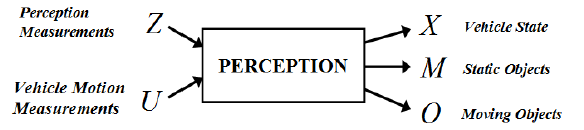
\includegraphics[scale=0.5]{img/fig:perception:cycle}
     \end{tabular}
   \caption{Perception cycle (adapted from \cite{VU-2009-454238})}
   \label{fig:perception:cycle}
 \end{figure}

In the next sections we are going to see in more details the approaches used in robotics research to tackle the localization and mapping and tracking of moving objects issues.

\subsection{SLAM}
SLAM (Simultaneous Localization and Mapping) is a process created to solve concurrently the \textit{mapping} and \textit{localization} problems\cite{VU-2009-454238}. In this approach it is assumed that the initial position of the ego-robot is unknown. 

In such process, the observation acquired by the robot's sensor must be used for estimation. The sensor readings should be enough to obtain the robot's \textit{localization}. That localization coordinates must be mapped into the current map of the environment. 

This model requires a precise \textit{mapping} of the environment. This precision is required due to parallel actions performed by the robot: moving itself in the scene (which changes the environment from the robots perspective) and localizing the robot at the same time, and as the robot motion is performed in a continuous space, any interference in the measurements are accumulated and can affect severely its localization estimation, diverging the calculated position from the real position. An Input-processing-output scheme can be seen in the Figure \ref{fig:perception:slam}.

\begin{figure}[h]
   \centering
     \begin{tabular}{lr}
       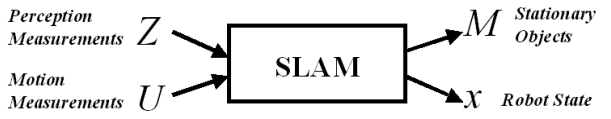
\includegraphics[scale=0.9]{img/fig:perception:slam}
     \end{tabular}
   \caption{SLAM process (adapted from \cite{Wang04a})}
   \label{fig:perception:slam}
\end{figure}

It is SLAM process responsibility to find out how to move in a certain environment having only noisy and incomplete measurements and without dynamic objects. Although, those constraints concerns just one set of application. For instance robots that are used for mining.

In the SLAM process knowing the positions that can be assumed by the robot is essential and necessary so that the robot can assume acceptable/non-occupied positions. This is done by observing the environment through the sensors and creating a spatial relationship among the static objects in this space \cite{iyengar1991autonomous}.

The robot actions are subject of physical interferences as well. It can be affected by the kind of terrain in which the robot is moving. Bringing it to the spotlight of some researchers that evaluate the slippage in direction changes at for robots that moves at high speed \cite{DBLP:conf/icra/LenainTHM11}. 

Thus, \textbf{inertial} factor plays a key role in determining how reliable the robot movements are. Other properties affects inertia such as: balance, weight distribution, grip condition, type of movement, etc. All those properties bring an imprecision factor into the movement performed by a robot. 

The output of the SLAM process is the robot state $x$ and the stationary objects map $M$, process represented in the Figure~\ref{fig:perception:slam}, captured by the \textit{perception} sensors \cite{iyengar1991autonomous}.

\subsubsection{Map representation}

Map representation is a key point to solve some of the problems related to scene understanding. Thus, the type of representation chosen can be the underline bases to achieve good results.

There exist several possible types of map that can be used to represent the robots surrounded environment. Among the alternatives for map representation, three of them gained importance, which are: \textbf{direct}, \textbf{grid} and \textbf{feature-based} \cite{Wang04a}.

\paragraph{Direct}

The direct map representation, is nothing but a straightforward representation of a sensor reading. 

This technique is frequently used in RADAR-like sensors. It depicts the point of impact of each beam (or radio wave frequency depending on the sensor) in an image. Binary image is enough to represent such images, it is easy and fast to build, can be extremely oscillating depending on the type of the sensor and the deployment depending on the quality of the sensors.

This representation uses only range measurements (\textit{e.g.} sonar, laser, etc.), this kind of representation is very convenient due to its simplicity. 

A research conducted by university of North York \cite{Lu:1997:GCR:591441.591464} focused their studies in the this issue. The fundamental problem was to obtain a local map from multiple reading, in such way that the resulting map was accurate. Those readings were done by a ego-vehicle able to move in the scenario. The scenario perceived by the robot can be seen in the Figure \ref{fig:mapping:direct:result}.

Those readings were performed by a single robot and its position was calculated based in informations provided by the IMU.

The result can be seen in the Figure \ref{fig:mapping:direct:result}. On the left image we have the original mapping, created with raw information and without any kind of filtering or preprocessing. On the right image, we have a map built with scan alignment technique\cite{Lu:1997:GCR:591441.591464}. On the second image we can see more sharp vertex and a precise alignment in the edges without mispositioned lines.

\begin{figure}[h]
\centering
	\begin{tabular}{lr}\\
		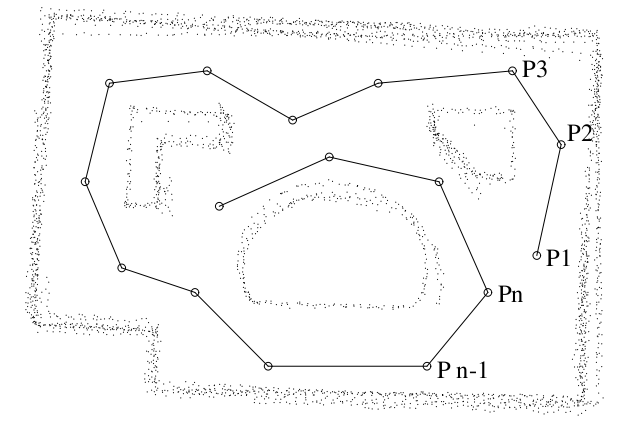
\includegraphics[width=0.5\columnwidth]{img/fig:mapping:direct:a} &
		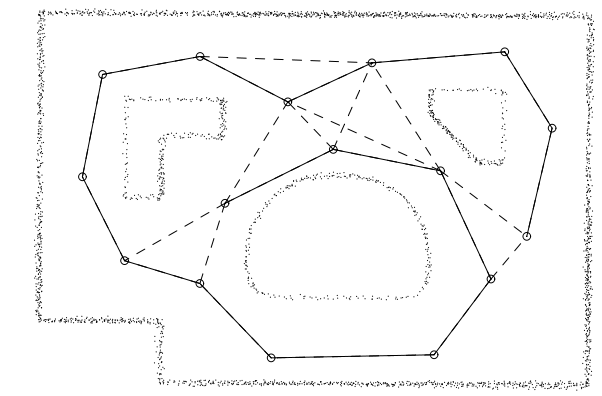
\includegraphics[width=0.5\columnwidth]{img/fig:mapping:direct:b}
	\end{tabular}
	\caption{Direct mapping result ( source \cite{Lu:1997:GCR:591441.591464} )}
	\label{fig:mapping:direct:result}
\end{figure}

Despite the good result obtained by scan alignment, it is not necessary in our approach, since we are not worried about building a map of the environment. 

\paragraph{Feature-based}

Another way to perceive the environment is the feature-based representation. In this type of map we use primitive shapes (\textit{e.g.} circles, lines, dots, ..) to represent the environment and its obstacles.

Several well known methods for detecting those features are available. Hough-transform, SIFT are good examples. 

Hough-transform is able to give us equation of lines that are part of the image. One good application for such method is to detect the edges of a road (left and right borders). By having an image of a plane road where the borders reach infinity, the Hough-transformation is capable to detect the line equation that represents the edges \cite{Ballard:1987:GHT:33517.33574}.

Scale-invariant feature transform (SIFT) detect similar points between two images, even if these similar points change in scale, noise, rotation or illumination \cite{Lowe:1999:ORL:850924.851523}.

Those methods are capable of detecting some features of an image and do a partial representation of its characteristics. 

The representation of the environment is not complete and it is subject to failures after applying the previous techniques.

This imprecise representation may generate false interpretation of the environment, that is why applying this kind of representation is not safe when ADAS is the goal platform.

\paragraph{Grid-based}
\label{ch02:gridbased}

Occupancy Grid is based on a multidimensional field that maintains the occupancy state information in a cell \cite{Elfes:1989:UOG:68491.68495}. Those cells are built in a regular size, and the number of cells which compose the grid is algorithm dependent.

By changing the size of the cells we can give more or less precision for the representation changing the resolution of the grid, which is reduce or increasing the size of the cell.

At the same time the Occupancy Grid, also known as \textit{certainty grids}, is effective in data representation it is also effective in representing sensor fusion information with it. 

Occupancy grid can be used as well to represent 3D environments, as was demonstrated in a small submersible craft, that looks for old battleships in the bottom of the ocean\cite{DBLP:journals/aim/Moravec88}.

One variation of the occupancy filter - The Bayesian Occupancy Filter(BOF) \cite{coue:inria-00182004} - contains the velocity and the probability distribution in Bayesian framework.

Representing continuous space when dealing with the uncertainty of an action of a mobile robot is extremely demanding in terms of resource usage, either in terms of processing power or memory allocation.

Thus, targeting to amortize the computational requirement for the uncertainty in the displacement of a robot, discretization models are used, Occupancy Grid\cite{Elfes:1989:UOG:68491.68495} is one of the former models proposed to tackle this issue.

This kind of representations is done with multi-dimensional vectors and results in a bird-eye view of the discretized map obtained by the perception sensor Figure \ref{fig:grid:continuous:discretized}.

\begin{figure}[h]
\centering
	\begin{tabular}{lr}\\
		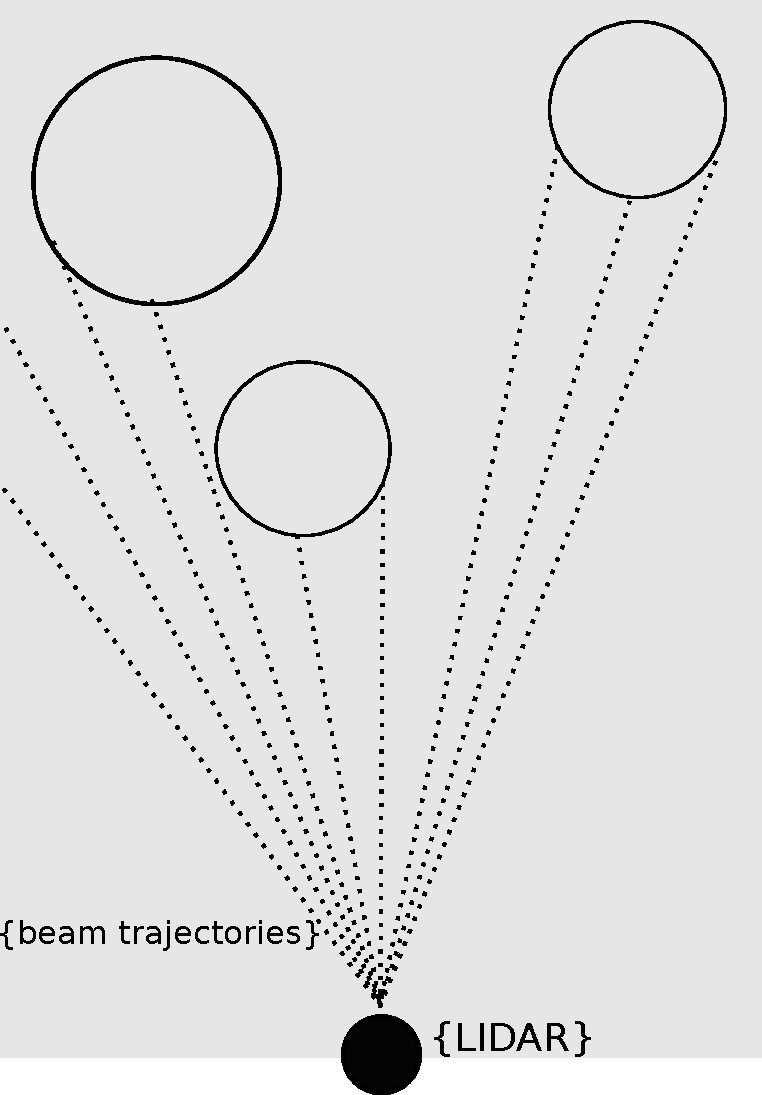
\includegraphics[width=0.25\columnwidth]{img/fig:motion:impactpoint:01} & %fig:grid:continuous
		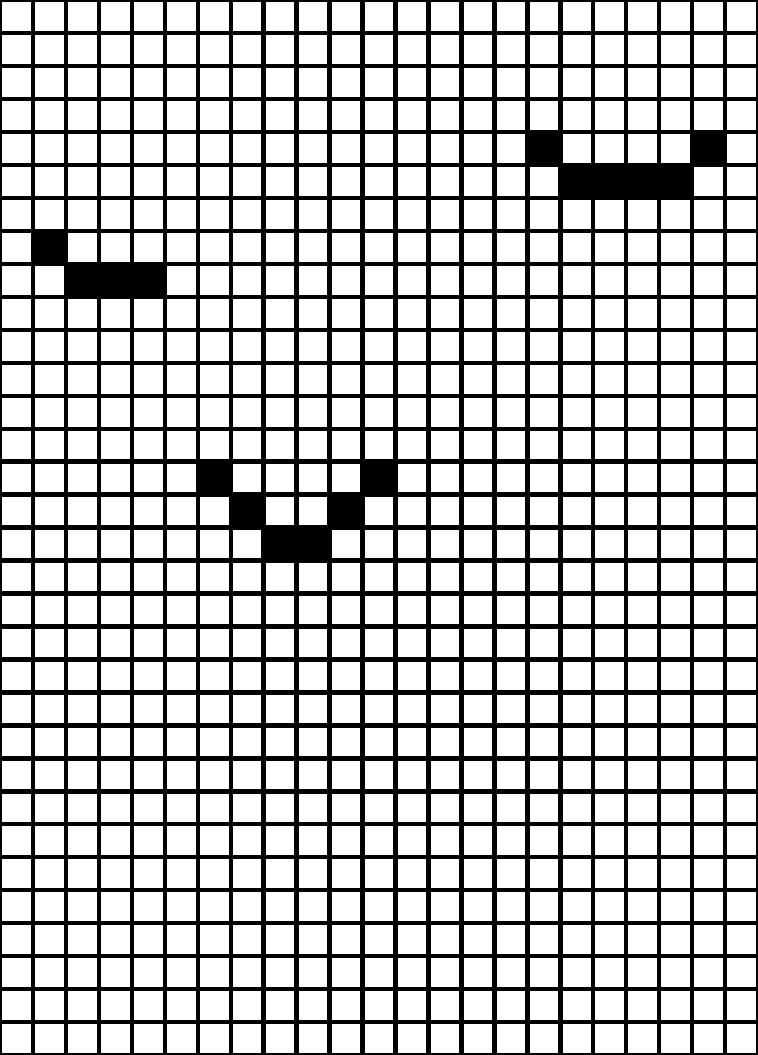
\includegraphics[width=0.25\columnwidth]{img/fig:motion:impactpoint:02} %fig:grid:discretized
	\end{tabular}
	\caption{Continuous \& discretized representation of a map}
	\label{fig:grid:continuous:discretized}
\end{figure}

In the grid framework each cell $C$ can be assigned have its state $\phi(C)$ configured to binary domain, so, either the current state of the cell is \textit{occupied} or it is \textit{free}, in this paper we state that the value $1$ represents the occupied state and $0$ a $free$ space Equation \ref{eq:binarycell}. A different domain may be used in the grid, for instance to represent random variable with a probability of occupancy of the cell (Section~\ref{sec:sensor:fusion}).

\begin{equation}
P(\phi(C)=1) + P(\phi(C)=0) = 1
\label{eq:binarycell}
\end{equation}

This model can be extended to a more general model coined as \textit{inference grids} that encapsulate multiple properties\cite{Elfes:1989:OGP:916528}.


\subsubsection{Didactic example}

In SLAM, our main concern is to localize ourselves and the static objects in the surrounding environment. 

Intending to simplify the perspective of this problem, we will generate a scenario that will be used in analogy to the formula and may help the reader to absorb the intuition behind the formalization.

\paragraph*{Lost Robot} is positioned arbitrarily in a finite unknown space. This is a classical 4 wheel robot. This same robot is subject to any kind of random forces and terrain condition. 

Suppose we send a command to the robot to move one centimeter ahead, how do we ensure that he really changed one centimeter? Suppose that without observing the last position of the robot we send another command to move another centimeter ahead, what would be the consequences? 

Every time we actuate in the robot without checking/knowing the real position, the uncertainty on localization grows, and the number of possible new positions that can be assumed by the robot increases exponentially.


\subsection{DATMO}

Detection and Tracking of Moving Objects (DATMO) was initially studied by radar tracking systems researchers \cite{qadeerthesis}. In RADAR technology only moving objects are visible, unless the RADAR itself is moving. This provides a simple classification, by assuming that all objects detected by the RADAR are moving objects. The same does not happen with laser scanners. 

In laser scanners all objects are visible independently on their state, so static and dynamic objects are included in the representation. Thus, it is a responsibility of a higher level process to classify those objects, in any kind of grouping types: static x dynamic, cars x motorcycles, cars x people, etc.

DATMO is process that encapsulates only moving objects observations. It is on charge of DATMO to detect and track those objects. It is a generic process definition and not a technique. Thus, several researchers have been proposing techniques to solve it throughout the years.

\begin{figure}[h]
   \centering
     \begin{tabular}{lr}
       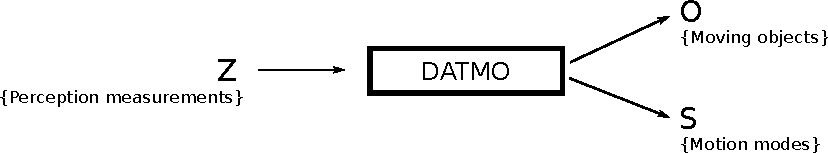
\includegraphics[scale=1.0]{img/fig:datmo:process}
     \end{tabular}
   \caption{DATMO process (adapted from \cite{Wang04a})}
   \label{fig:datmo:process}
 \end{figure}

Wang \cite{Wang03onlinesimultaneous} defined the DATMO tasks as:

\begin{itemize}
\item Detect and initializa new objects;
\item Motion modeling;
\item Data association;
\item Merge coalescent objects;
\item Remove the objects that moved outside of the FoV of the sensor;
\end{itemize}

Researchers considered SLAM and DATMO as two independent and different problems that should be solved separately. \textit{Wang} was the first researcher to put in evidence the similarities between both problems and propose simultaneous processing of those tasks\cite{Wang03onlinesimultaneous}. The SLAM and DATMO mutual cooperation is depicted in the Figure~\ref{fig:datmoslam:loop}.

\begin{figure}[h]
   \centering
     \begin{tabular}{lr}
       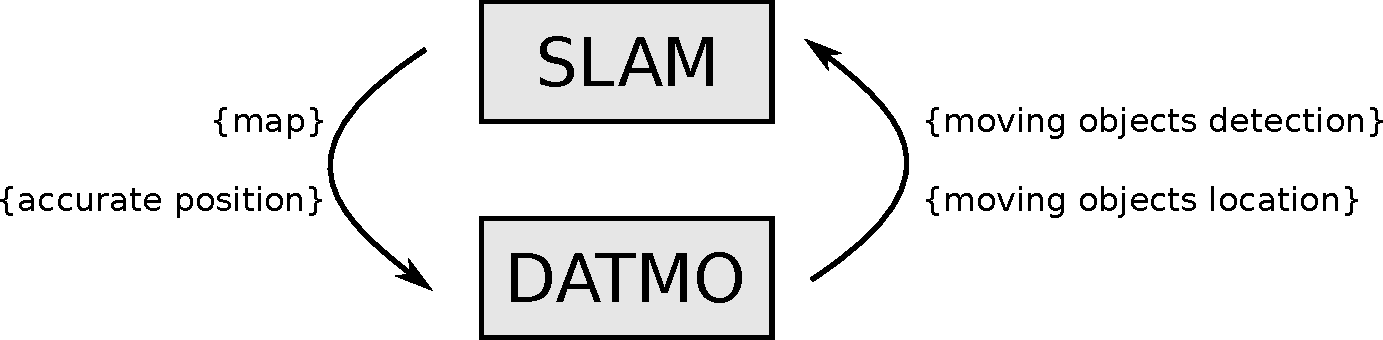
\includegraphics[scale=0.5]{img/fig:datmoslam:loop}
     \end{tabular}
   \caption{SLAM and DATMO: Mutual benefit (adapted from \cite{VU-2009-454238})}
   \label{fig:datmoslam:loop}
 \end{figure}

As result, the SLAMMOT term was coined and a derivation of the SLAM formula with DATMO was created to simplify the process of tracking. The experiments showed that solving simultaneously the SLAM with DATMO increased the quality of the algorithm results comparing them with their results as individual processes \cite{Wang02simultaneouslocalization}. In the other hand, the process gets much more complex and computational expensive. In the figure \ref{fig:slammot} we can see the input-process-output schema for the SLAMMOT process.

\begin{figure}[h]
   \centering
     \begin{tabular}{lr}
       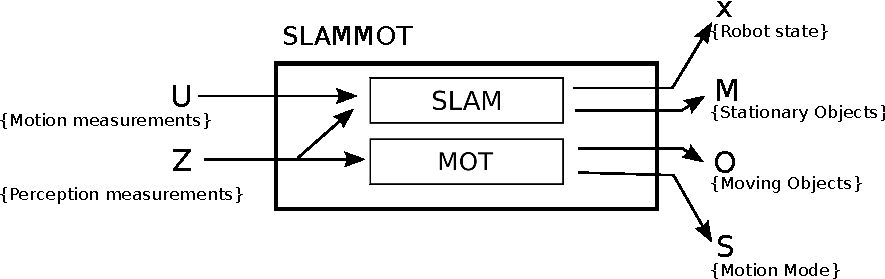
\includegraphics[scale=0.9]{img/fig:slammot}
     \end{tabular}
   \caption{SLAMMOT composition (adapted from \cite{Wang04a})}
   \label{fig:slammot}
 \end{figure}

Nowadays, the challenging in DATMO is to turn it into a reliable process in a highly dense and highly dynamic environments.

\section{Mutual cooperation: SLAM and DATMO}

\textbf{Scenario 1}: in a simpler scenario we can have a robot that moves in an environment, where all objects in its surroundings are static. The robot is the only element present in the environment that is moving.

In this case, the static environment is everything that the robot can perceive. So the robot should use these information to build a map of the navigable path (SLAM).

\textbf{Scenario 2}: suppose the robot is moving in an overly crowded environment, with different type of objects (cars, pedestrian, trucks, bicycle, motorbikes, etc.), static and moving objects are mixed. Which object to use as static objects (\textit{e.g.} to build the map) and which to use as dynamic (\textit{e.g.} to calculate the risk of collision)? 

In the \textbf{Scenario 2}, it is much more complicated to obtain any information from the environment.

This leads us to one conclusion: it is hard to do risk analysis when you do not know the objects of the scene. In addiction, it is intrinsically hard to find the motion model of a specific object in the scene(behavior analysis).

Thus, as a stepping stone we can perform the dynamic and static environment classification. This solves part of the problem, by classifying the environment in two categories. This will help to:

\begin{enumerate}
\item Build the map (which is not the our goal)
\item Perform DATMO
\item Perform risk assessment (Section~\ref{sec:riskassessment})
\end{enumerate}

The scene understanding usually implicates in distinguish different elements in the scene, objects or even types of objects. This distinction can be done by using the objects' features(\textit{e.g.} color, shape, etc.), path perceived or even its behavior (motion pattern behavior). 

\section{Problem addressed}

In this chapter we have seen the concepts required to understand the applicability of the problem addressed in this document. We introduced the most common approaches and terminologies adopted in the robotics field. 

In this document we will detail our approach to perform a fast and high level classification. Classifying dynamic parts in an image by using the minimum amount of video frames. The details of our methods will be explained in next sections.

%multimodels, importance sampling, prior map knowledge